% -----------------------------------------------------------------------------
\documentclass[a4paper]{artikel3}
% -----------------------------------------------------------------------------
\paperheight = 29.70 cm  \paperwidth = 21.0 cm  \hoffset        = 0.46 cm
\headheight  =  0.81 cm  \textwidth  = 15.0 cm  \evensidemargin = 0.00 cm
\headsep     =  0.81 cm	 \textheight = 9.00 in  \oddsidemargin  = 0.00 cm					
% -----------------------------------------------------------------------------
\usepackage{enumerate}
\usepackage{amsfonts}
\usepackage{amsmath}
\usepackage{url}
\usepackage{graphicx}
\usepackage{float}
\usepackage[font=small,labelfont=bf]{caption}
\usepackage{setspace}
\usepackage{booktabs}
\usepackage[pdfpagemode=None,
		    colorlinks=true, 
		    urlcolor=blue, 
		    linkcolor=blue, 
		    citecolor=blue, 
		    pdfstartview=FitH]{hyperref}
% -----------------------------------------------------------------------------
\newtheorem{thm}{Theorem}
\newtheorem{cor}[thm]{Corollary}
\newtheorem{lem}{Lemma}
\newtheorem{prop}{Proposition}
\newtheorem{definition}[thm]{Definition}
\newtheorem{rem}[thm]{Remark}
\newtheorem{exm}[thm]{Example}
% -----------------------------------------------------------------------------
\newcommand{\norm}[1]{\left\Vert#1\right\Vert}
\newcommand{\abs}[1]{\left\vert#1\right\vert}
\newcommand{\set}[1]{\left\{#1\right\}}
\newcommand{\Real}{\mathbb R}
\newcommand{\eps}{\varepsilon}
\newcommand{\To}{\longrightarrow}
\newcommand{\mb}[1]{\mathbf{#1}}
\newcommand{\gb}[1]{\text{\boldmath$#1$}}
\newcommand{\ov}[1]{\overline{#1}}
\newcommand{\mml}{\{}
\newcommand{\mmr}{\}}
\newcommand{\lh}[1]{\widehat{#1}}
\newcommand{\pname}[1]{\textsc{#1}}
\newcommand{\lc}[1]{\mathscr{#1}}
\newcommand{\lcs}[1]{\ov{\mathscr{#1}}}
\newcommand{\lco}[1]{\overline{\mathscr{#1}}}
\newcommand{\lch}[1]{\widehat{\mathscr{#1}}}
\newcommand{\spi}{\ell}
\newcommand{\zf}[1]{z(#1)}
\newcommand{\R}{\mathbb{R}}
% -----------------------------------------------------------------------------
\allowdisplaybreaks
\onehalfspacing
% -----------------------------------------------------------------------------
\begin{document}

% Title page
\begin{center}
{\Large \onehalfspacing \bf Solving Large-Scale Optimization Problems with ADMM}
\end{center}
\vspace{10pt}

% Use this if you work on your own and delete or comment over lines 72 - 77
%\begin{center}
%Hardworking Student\\
%{\textit{{\small{Aalto University School of Science, Department of Mathematics and Systems Analysis, 
%                 \{hardworking.student@aalto.fi\}}}}}
%\end{center}

% Use this if you work with a pair
\begin{center}
Anonymous Student, Hardworking Student\\ 
{\textit{{\small{Aalto University School of Science, Department of Mathematics and Systems Analysis\\
		         Aalto University School of Science, Department Computer Science\\ 
		         \{anonymous.student, hardworking.student\}@aalto.fi}}}}
\end{center}


\section{Background}

Here is some example text.

In this project, you will use the knowledge acquired in the course to develop a variant of the \emph{Alternating Direction Method of Multipliers} (ADMM) that can solve large-scale stochastic capacity expansion problems.

\section{Applications}


Here is an example how to add a Figure. Make sure the picture file is in the correct folder.

\begin{figure}[H]
\centering
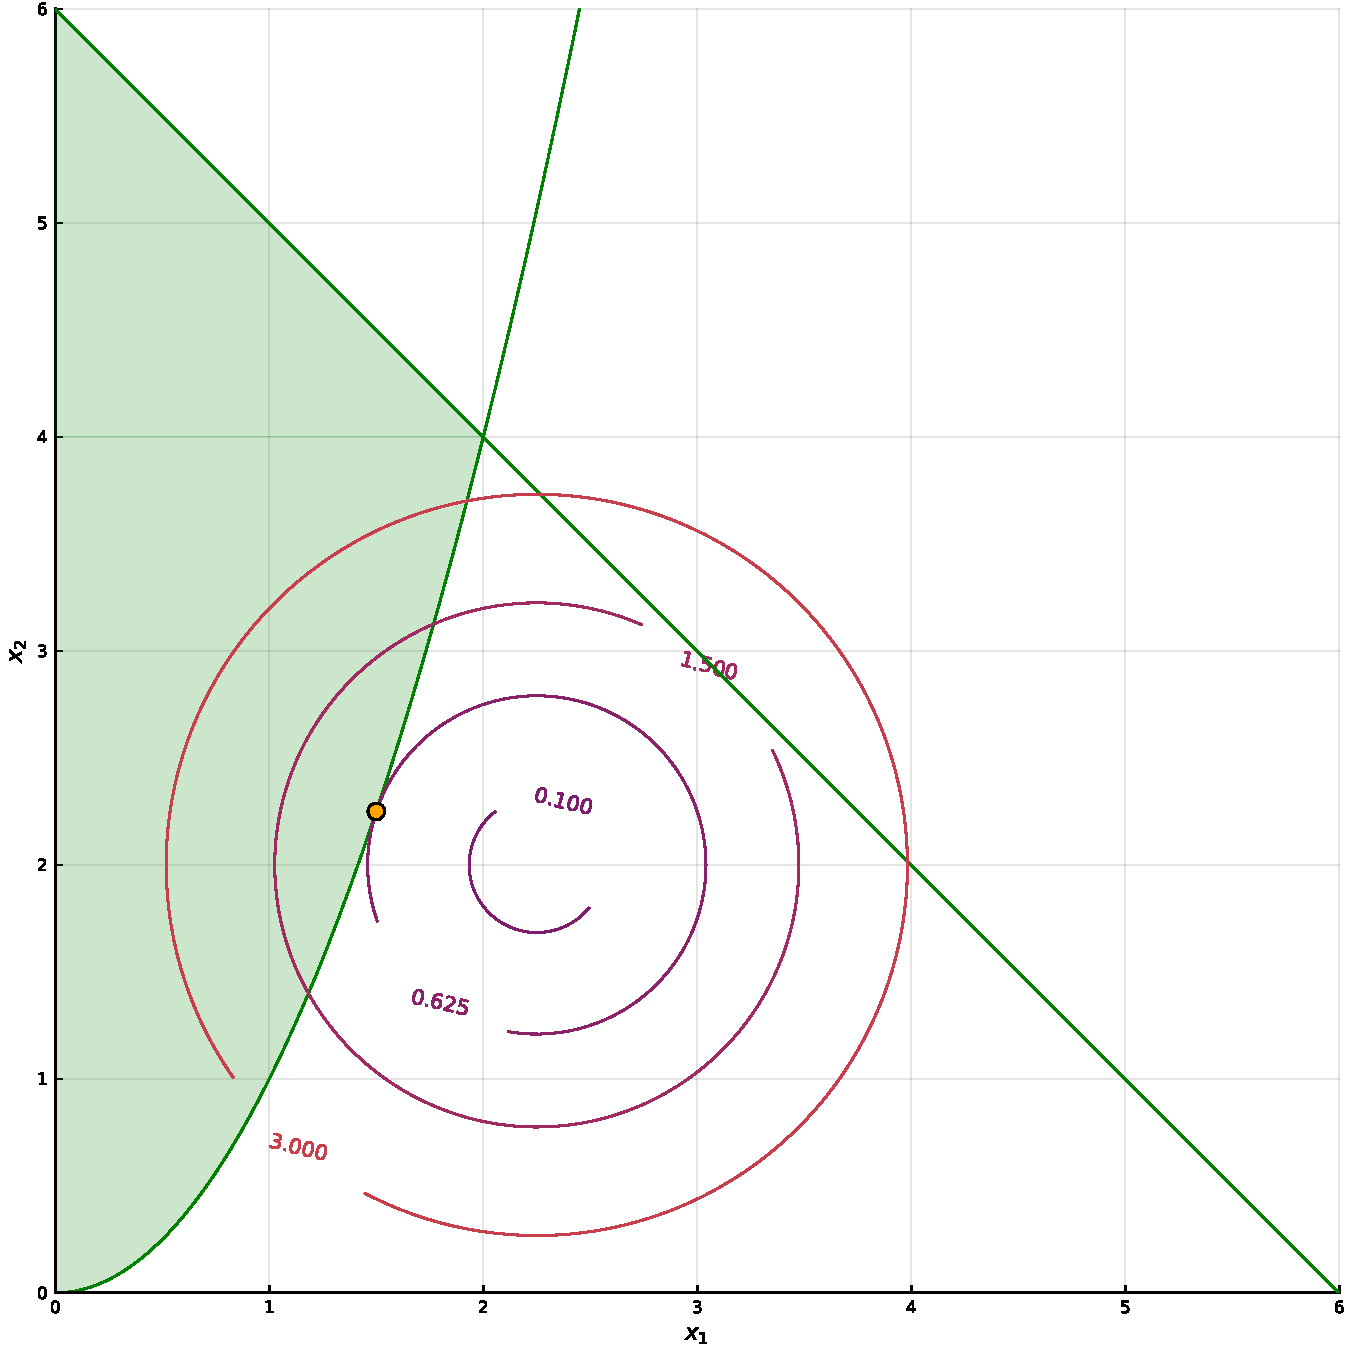
\includegraphics[scale=0.50]{Figures/example.pdf}
\caption{Plotting with Julia is fun when it works.}
\label{fig:1}
\end{figure}

You can refer to Figure \ref{fig:1} like this. 


Here is an example how to add a table if needed. 

\begin{table}[H]
\caption{Example table}
\label{tbl:1}
\centering
\begin{tabular}{l r r r}
\toprule
Value of $\rho$    &   Time   &   Iterations  &   Solution\\
\midrule
10    &  111.02  &  2  &  12.09\\
100   &   98.09  &  4  &  12.09\\
200   &  124.34  &  7  &  999.92\\
500   &   10.70  &  4  &  12.09\\
1000  &  234.01  & 10  &  12.34\\
10000 &  592.12  &  9  &  12.40\\
\bottomrule
\end{tabular}
\end{table}

You can refer to Table \ref{tbl:1} like this.

\section{Discussion and conclusions}

As can be seen in Table \ref{tbl:1}, the value of the penalty parameter $\rho$ ...



\end{document} 